%! Author = admin
%! Date = 2023/12/4

% Preamble
\documentclass[a4paper]{article}

% Packages
\usepackage[margin=1in]{geometry}
\usepackage[fontset=founder]{ctex}
\usepackage{anyfontsize}
\usepackage{graphicx}
\usepackage{amsmath}
\usepackage{amssymb}
\usepackage{mathabx}
\usepackage{multirow}
\usepackage{subfig}

\graphicspath{{../figures/}}

\title{\textbf{晶体管共射极单管放大器}}
\author{姚苏航\qquad PB22061220 \\ 庞宇乐\qquad PB22061166}
\date{实验时间: 2023年11月29日\qquad 座位号: 05}

% Document
\begin{document}
    \maketitle


    \section{实验目的}\label{sec:}

    \noindent{1.掌握放大器静态工作点的测量与调试方法。\cite{ed4}}

    \noindent{2.学习放大电路的交流特性等性能指标的测量方法。}

    \noindent{3.掌握静态工作点与输出波形失真的关系,了解最大不失真输出电压的测量方法。}


    \section{实验原理}\label{sec:10}
    \begin{center}
        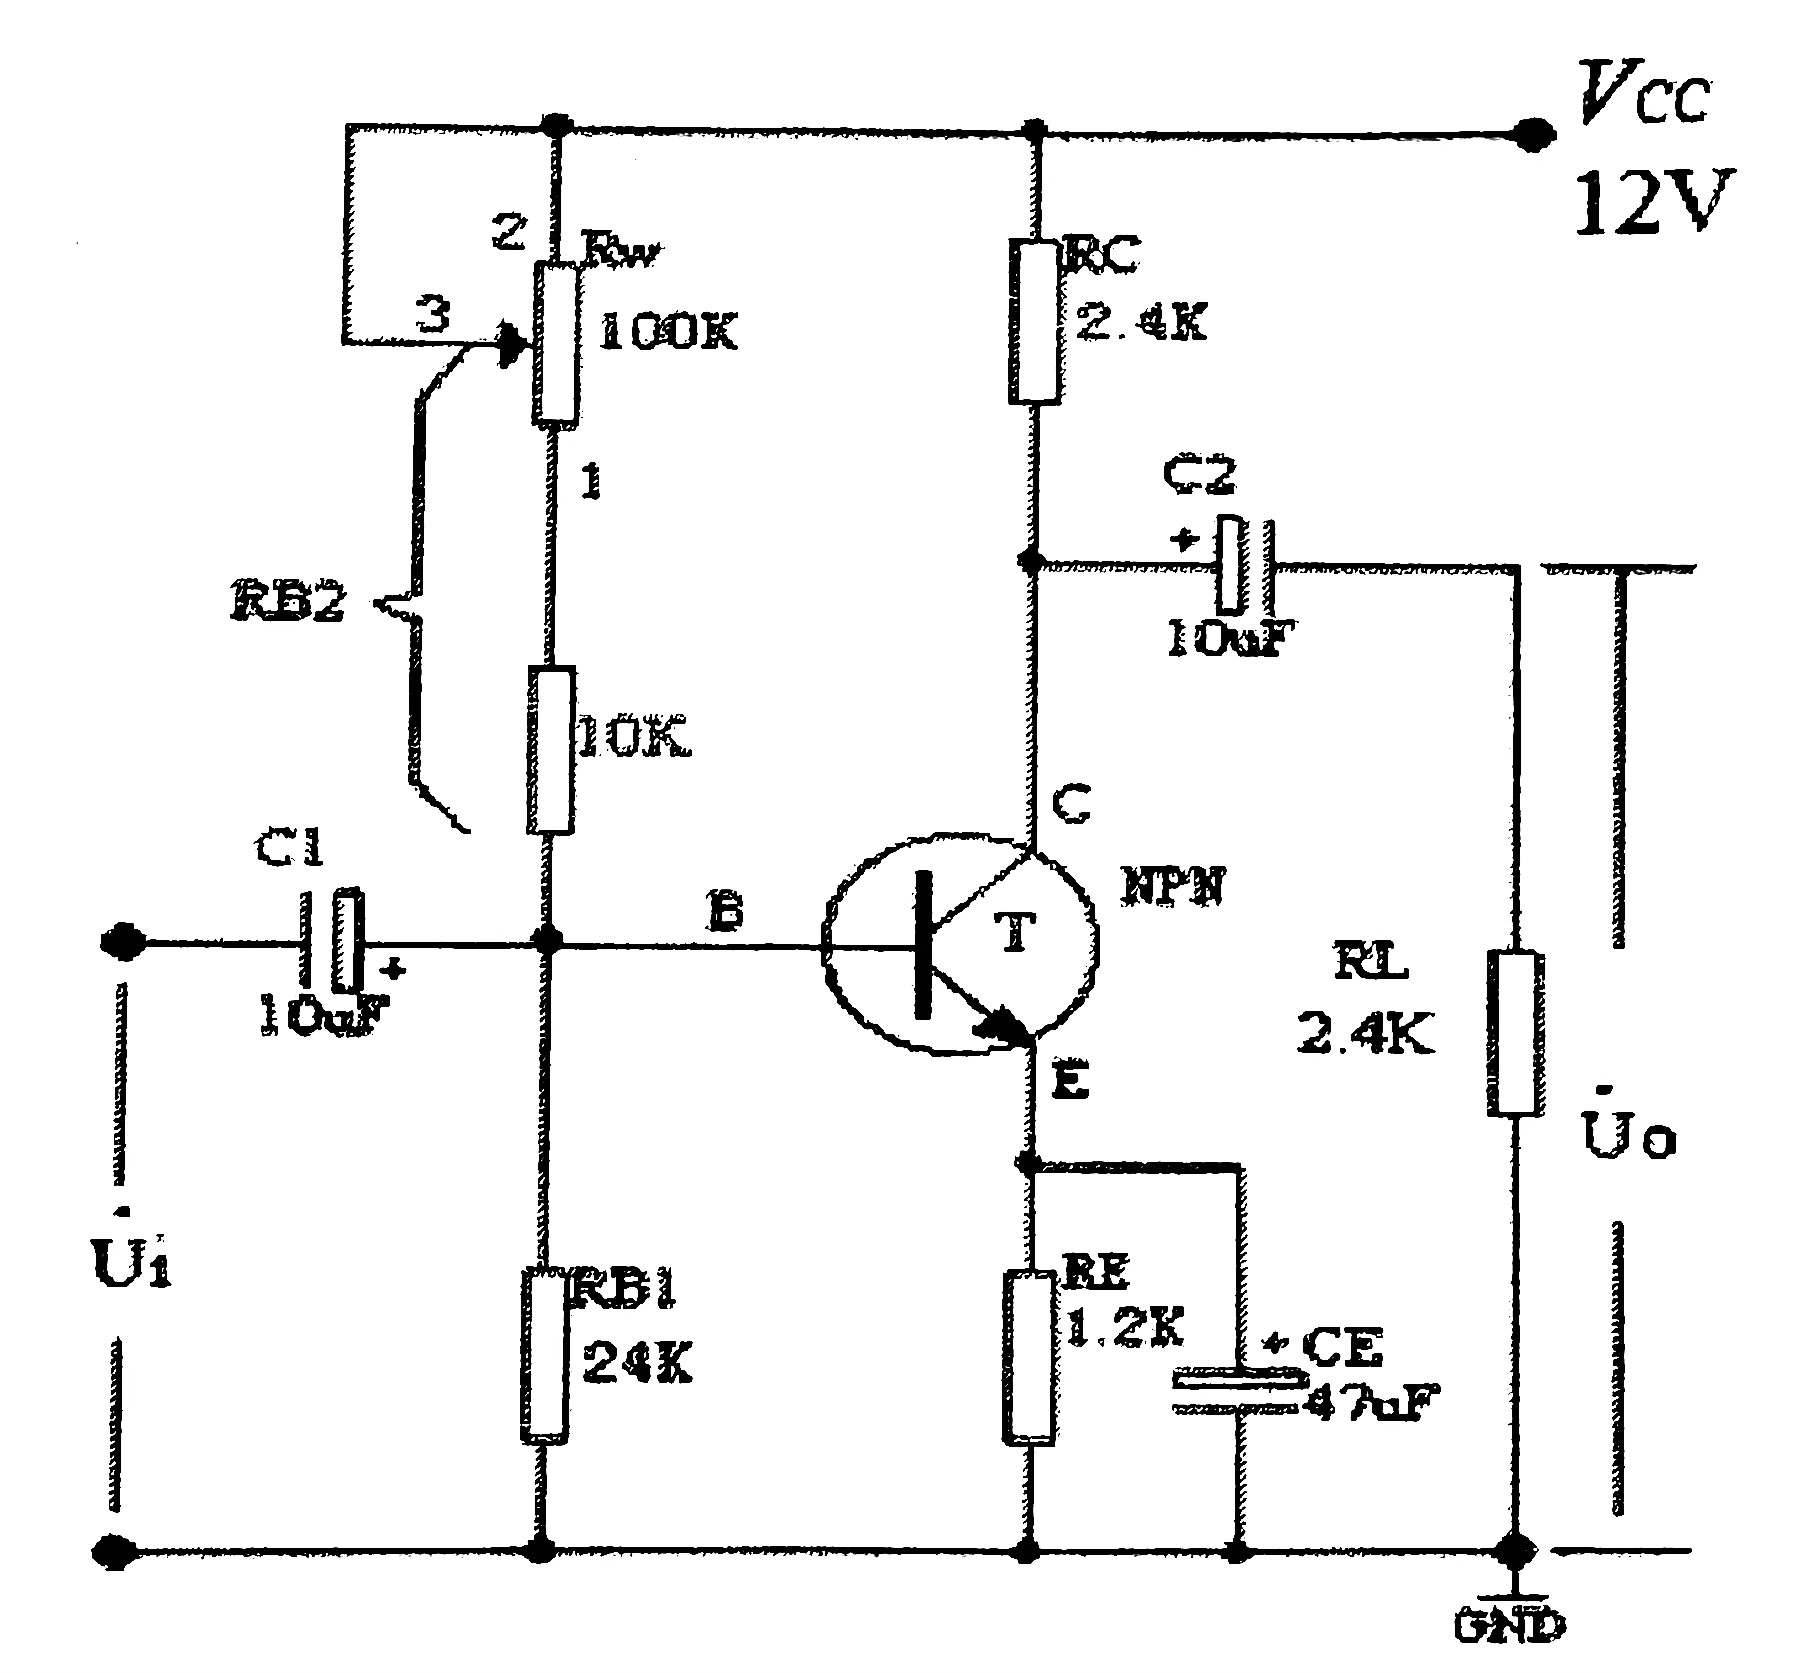
\includegraphics[height=150pt]{AC}\\
        {\small 图一:共射极单管放大电路}
    \end{center}

    {{图一为电阻分压式工作点稳定单管放大器实验电路图。其中偏置电路采用$R_{B1}$和$R_{B2}$组成的分压电路。$V_{CC}$作为集电极电源为电路提供能量,保证发射结正偏、集电结反偏。集电极电阻$R_C$将变化的电流转变成变化的电压,是电路具有电压放大能力。发射极电阻$R_E$引入负反馈稳定电路,稳定放大器静态工作点。耦合电容$C_1$和$C_2$隔离输入输出与电流直流的联系,同时能使信号顺利输入输出。}}


    \section{实验仪器}\label{sec:2}


    \section{测量静态工作点}\label{sec:3}

    \subsection{实验内容}\label{subsec:2}
    \begin{center}
        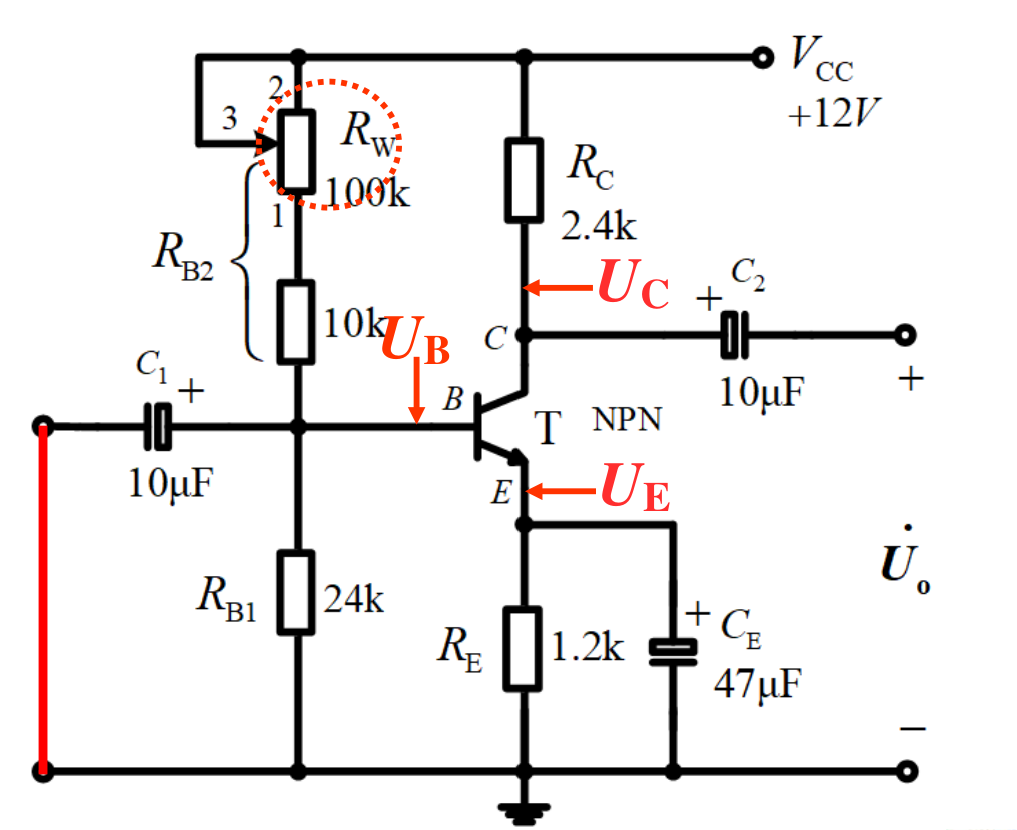
\includegraphics[height=150pt]{exp2}\\
        {\small 图二:实验电路}
    \end{center}

    \subsection{实验数据与误差分析}\label{subsec:3}

    \subsection{注意事项}\label{subsec:4}


    \section{测量电压放大倍数}\label{sec:4}

    \subsection{实验原理}\label{subsec:5}

    \subsection{实验内容}\label{subsec:6}

    \subsection{实验数据与误差分析}\label{subsec:7}
    \begin{center}
        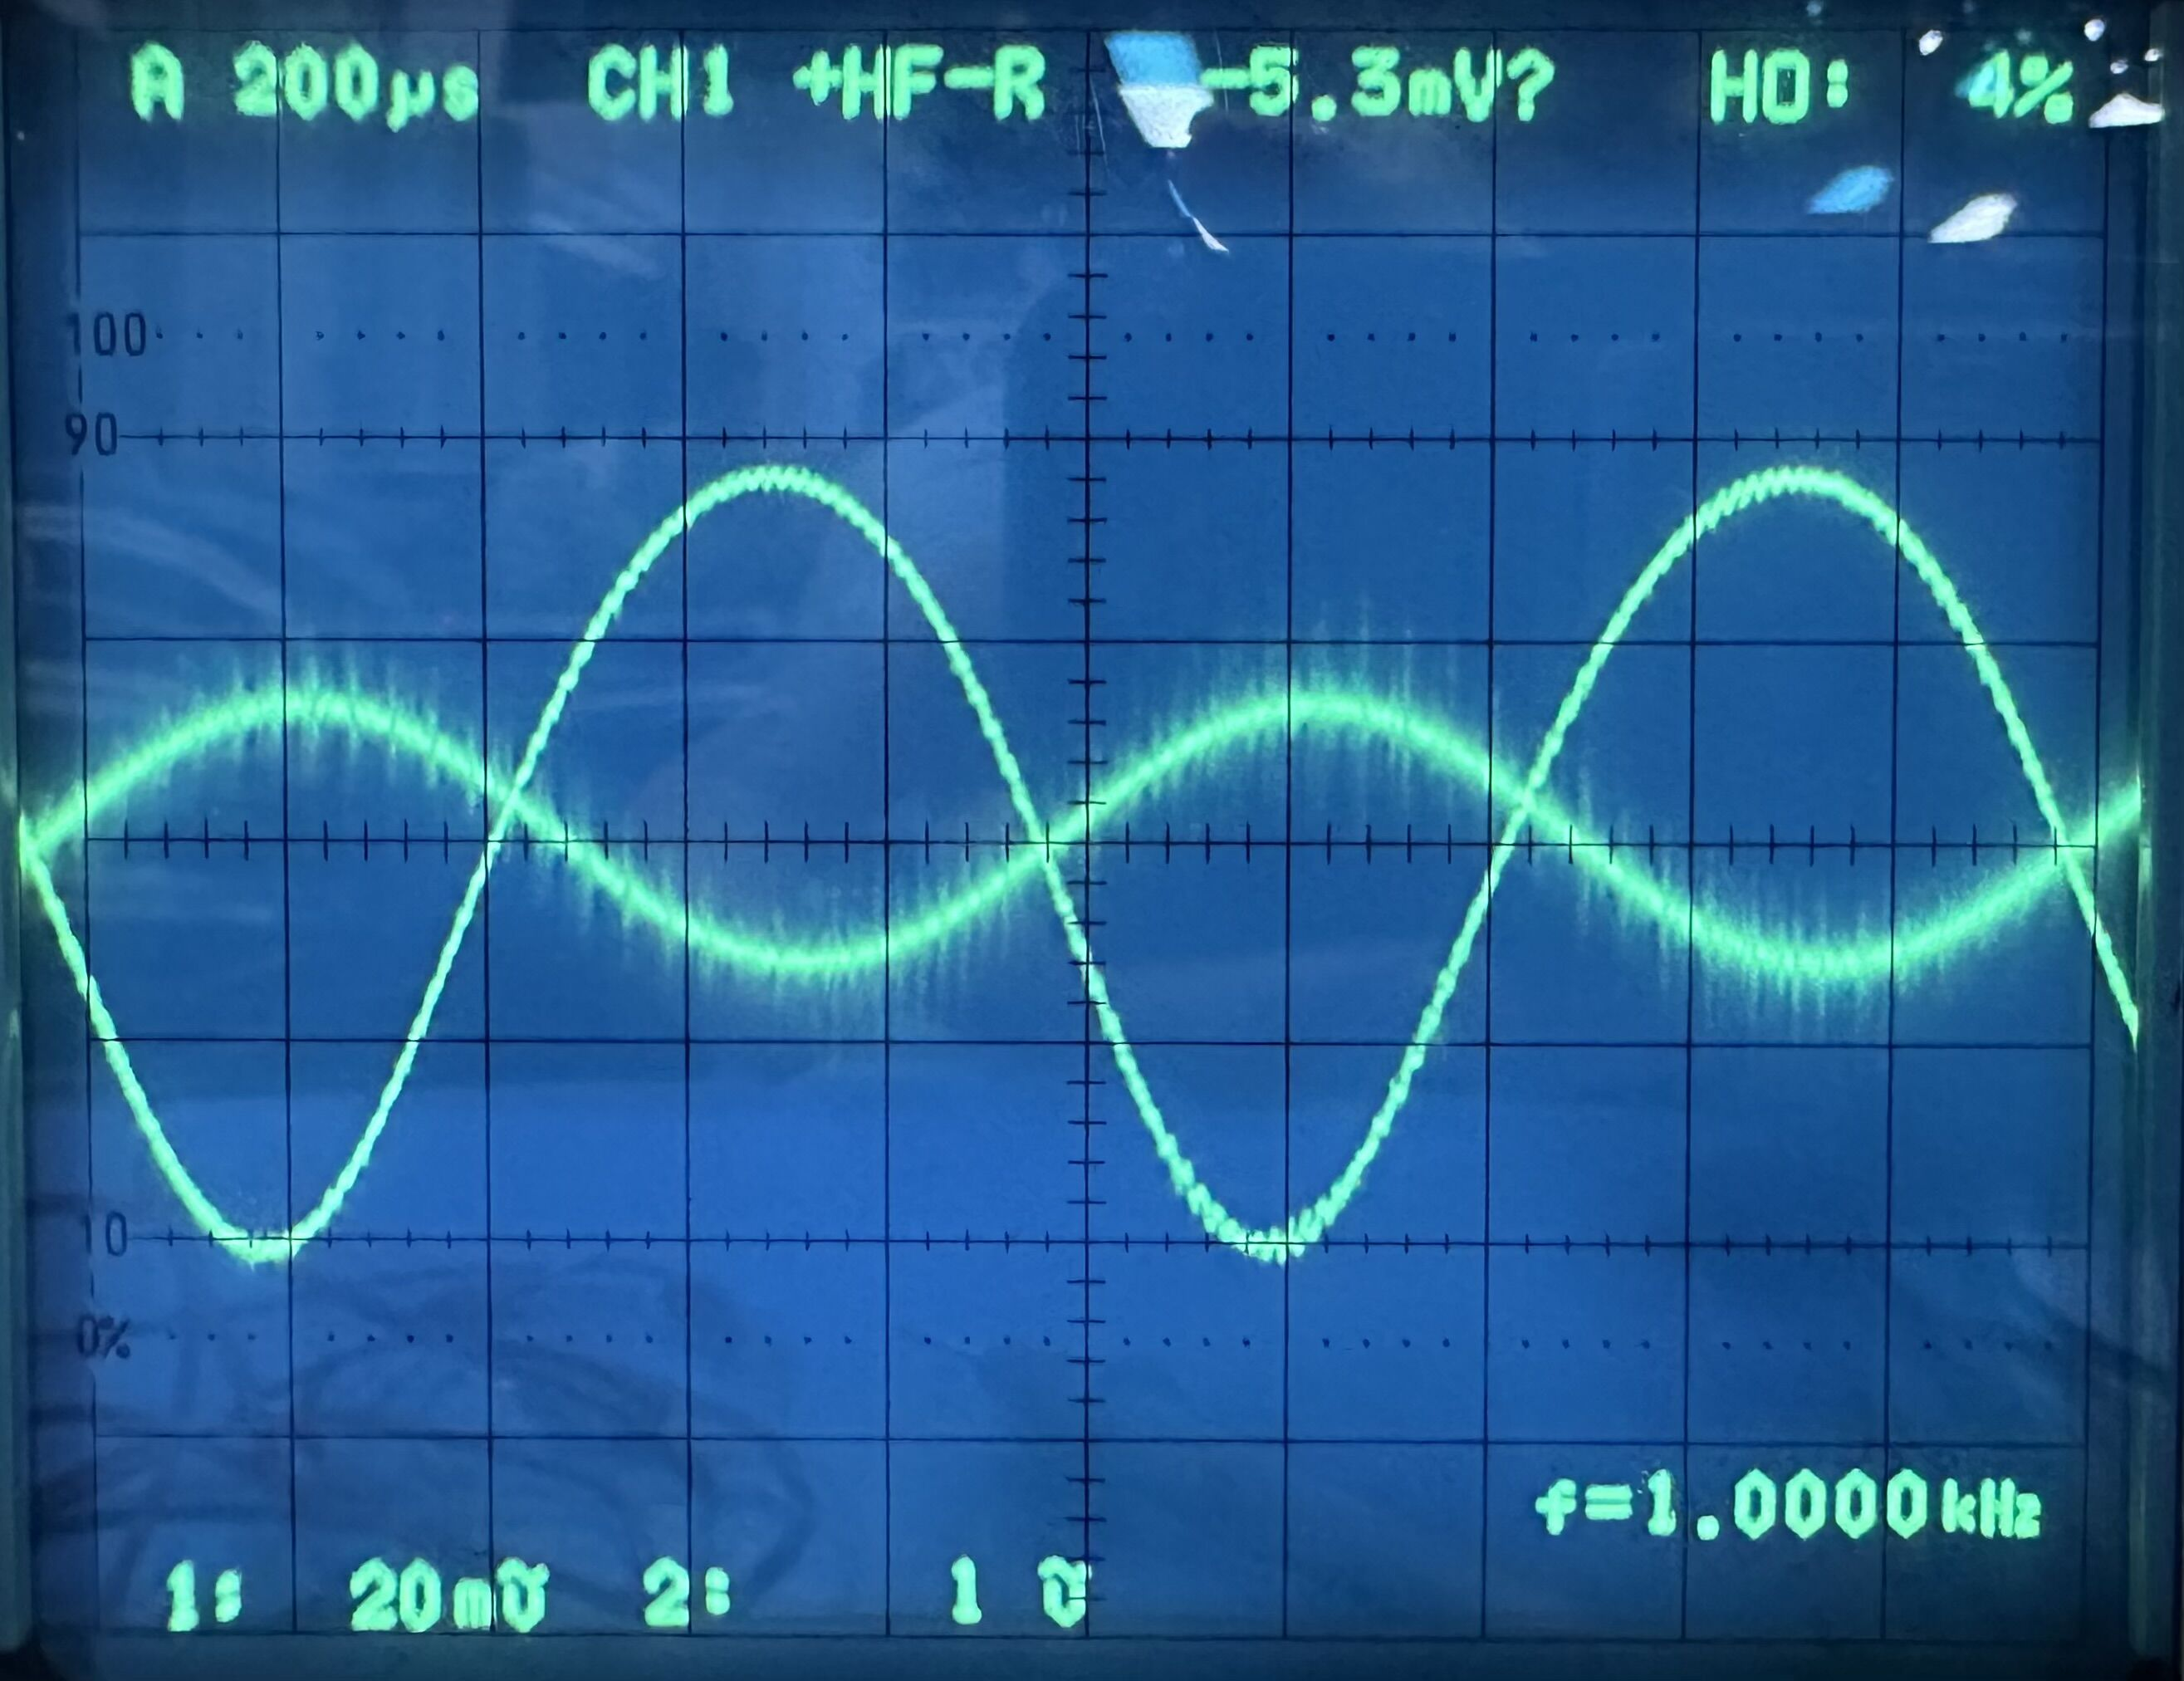
\includegraphics[height=130pt]{ref}\\
        {\small 图三:$u_o$和$u_i$的相位关系}
    \end{center}

    \subsection{注意事项}\label{subsec:8}


    \section{测量输入电阻和输出电阻}\label{sec:5}
    \begin{center}
        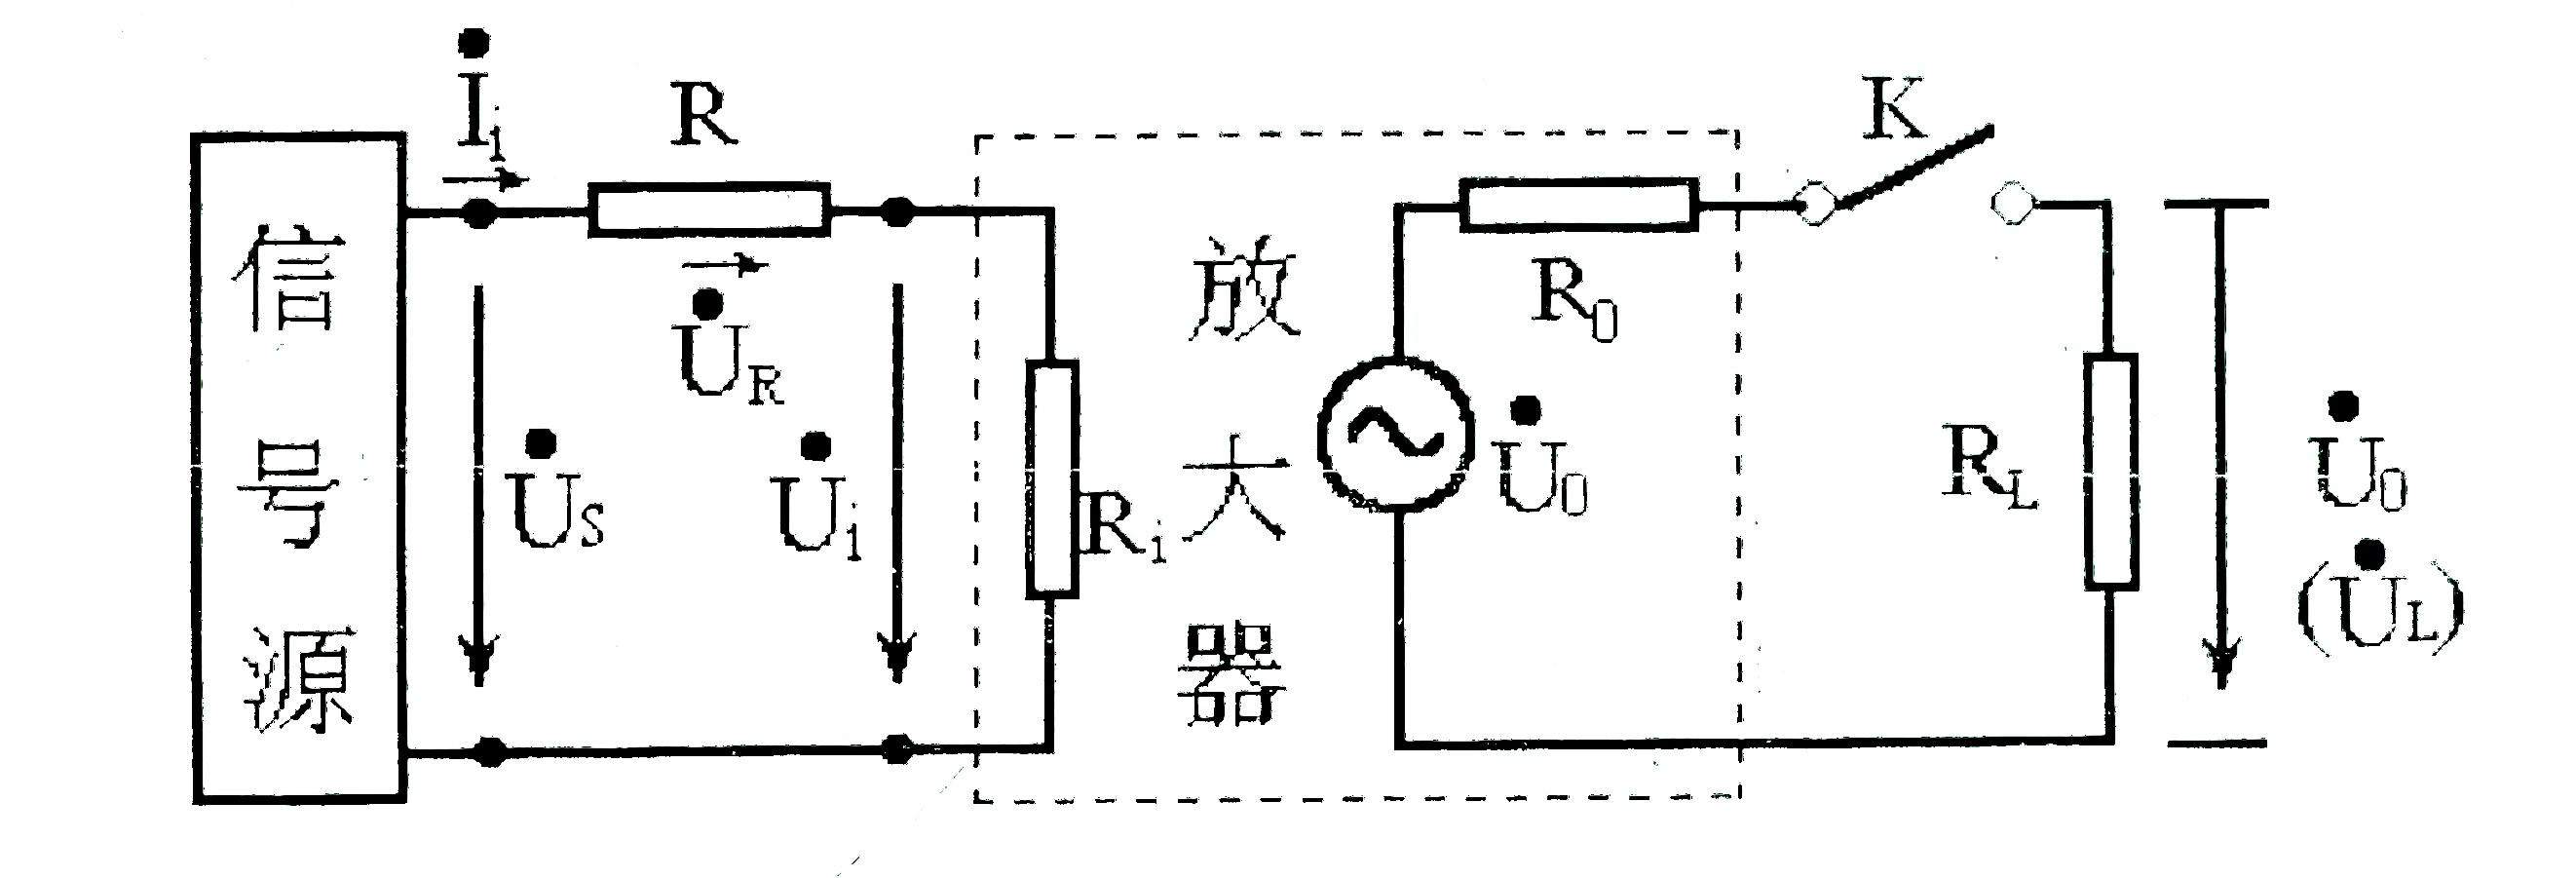
\includegraphics[height=80pt]{R}\\
        {\small 图四:实验电路}
    \end{center}

    \subsection{实验原理}\label{subsec:9}

    \subsection{实验内容}\label{subsec:10}

    \subsection{实验数据与误差分析}\label{subsec:11}

    \subsection{注意事项}\label{subsec:12}


    \section{测量幅频特性曲线}\label{sec:6}

    \subsection{实验原理}\label{subsec:13}
    \begin{center}
        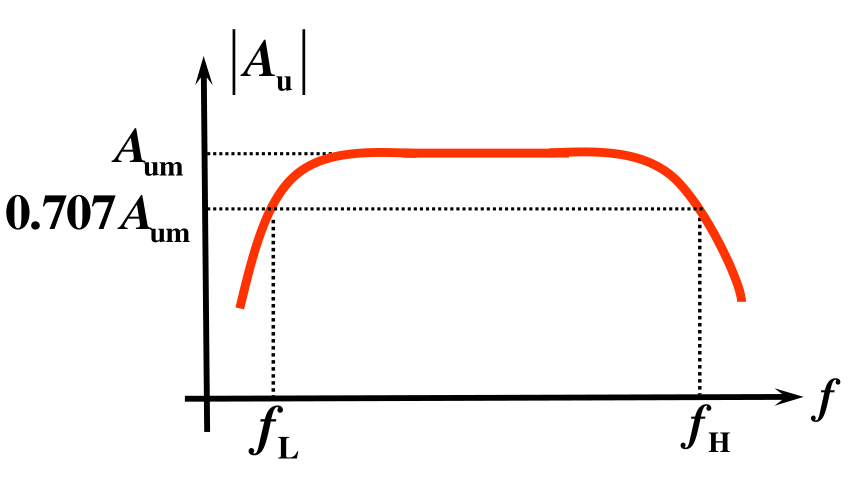
\includegraphics[height=120pt]{Af}\\
        {\small 图五:理想幅频特性曲线}
    \end{center}

    \subsection{实验内容}\label{subsec:14}

    \subsection{实验数据与误差分析}\label{subsec:15}
    \begin{table}[!t]
        \centering
        \begin{tabular*}{\textwidth}{@{\extracolsep{\fill}}|l|l|l|l|l|l|l|l|}
            \hline
            f/Hz     & 200    & 250    & 269    & 270    & 271     & 280    & 300    \\
            \hline
            $U_o$/V  & 0.442  & 0.492  & 0.512  & 0.513  & 0.514   & 0.52   & 0.534  \\
            \hline
            $U_i$/mV & 9.30   & 9.30   & 9.30   & 9.30   & 9.29    & 9.29   & 9.28   \\
            \hline
            |Au|     & 47.527 & 52.903 & 55.054 & 55.161 & 55.3281 & 55.974 & 57.543 \\
            \hline
        \end{tabular*}

        \begin{tabular*}{\textwidth}{@{\extracolsep{\fill}}|l|l|l|l|l|l|l|l|}
            \hline
            f/Hz     & 500    & 1000   & 3000   & 5000   & 10000  & 15000  & 20000  \\
            \hline
            $U_o$/V  & 0.619  & 0.678  & 0.709  & 0.713  & 0.717  & 0.717  & 0.717  \\
            \hline
            $U_i$/mV & 9.27   & 9.24   & 9.22   & 9.21   & 9.19   & 9.18   & 9.18   \\
            \hline
            |Au|     & 66.774 & 73.377 & 76.898 & 77.416 & 78.020 & 78.104 & 78.104 \\
            \hline
        \end{tabular*}

        \begin{tabular*}{\textwidth}{@{\extracolsep{\fill}}|l|l|l|l|l|l|l|l|}
            \hline
            f/Hz     & 30000  & 70000  & 100000 & 200000 & 300000 & 400000 & 470000 \\
            \hline
            $U_o$/V  & 0.716  & 0.705  & 0.693  & 0.638  & 0.568  & 0.498  & 0.459  \\
            \hline
            $U_i$/mV & 9.16   & 9.13   & 9.10   & 8.91   & 8.69   & 8.45   & 8.28   \\
            \hline
            |Au|     & 78.166 & 77.218 & 76.154 & 71.605 & 65.362 & 58.935 & 55.435 \\
            \hline
        \end{tabular*}

        \begin{tabular*}{\textwidth}{@{\extracolsep{\fill}}|l|l|l|l|l|l|l|l|}
            \hline
            f/Hz     & 475000 & 480000 & 485000 & 490000 & 495000 & 500000 & 700000 \\
            \hline
            $U_o$/V  & 0.458  & 0.456  & 0.455  & 0.451  & 0.448  & 0.445  & 0.349  \\
            \hline
            $U_i$/mV & 8.27   & 8.26   & 8.25   & 8.24   & 8.23   & 8.22   & 7.87   \\
            \hline
            |Au|     & 55.381 & 55.206 & 55.152 & 54.733 & 54.435 & 54.136 & 44.346 \\
            \hline
        \end{tabular*}\label{tab:table}
    \end{table}

    \begin{center}
        \includegraphics[height=200pt]{Graph1}\\
        {\small 图六:实际幅频特性曲线}
    \end{center}

    \subsection{注意事项}\label{subsec:16}


    \section{观察静态工作点对输出波形失真的影响}\label{sec:7}

    \subsection{实验原理}\label{subsec:17}
    \begin{figure*}[htb]
        \centering
        \subfloat[饱和失真与截止失真]{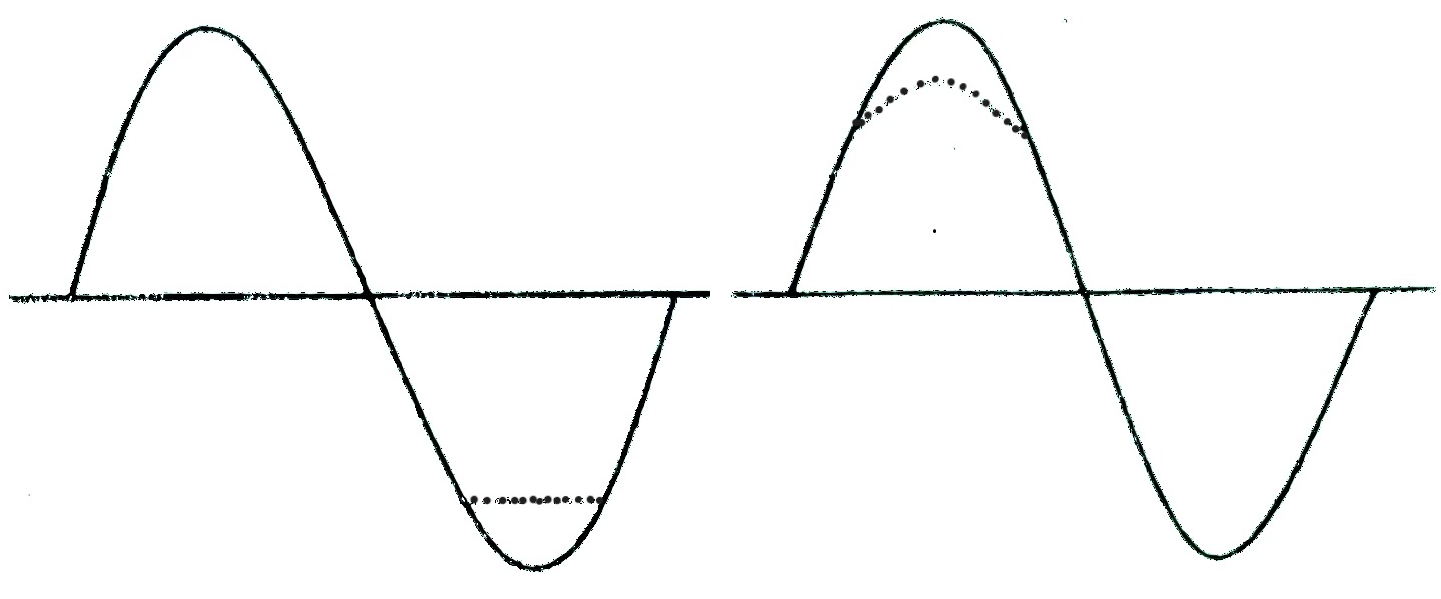
\includegraphics[height=100pt]{ID2}}
        \subfloat[电路参数对静态工作点影响]{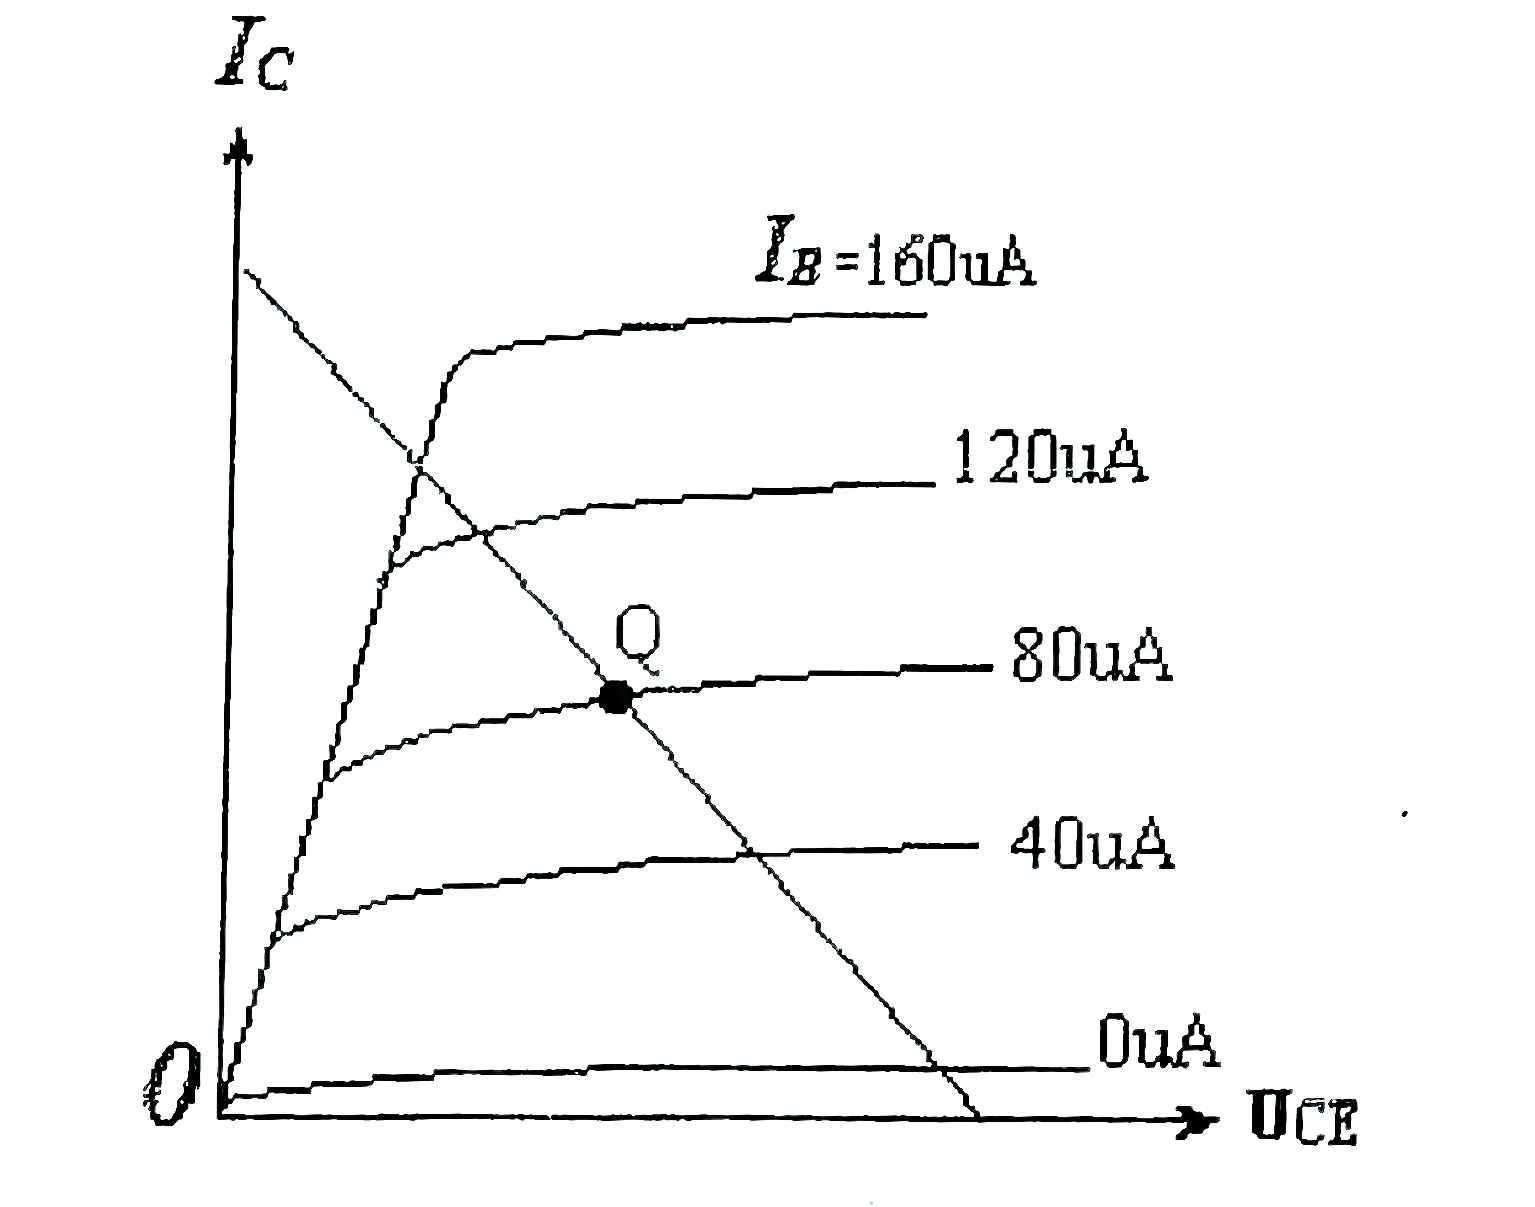
\includegraphics[height=100pt]{IU}}\\
        {\small 图七:理论图像}
    \end{figure*}

    \subsection{实验内容}\label{subsec:18}
    \begin{center}
        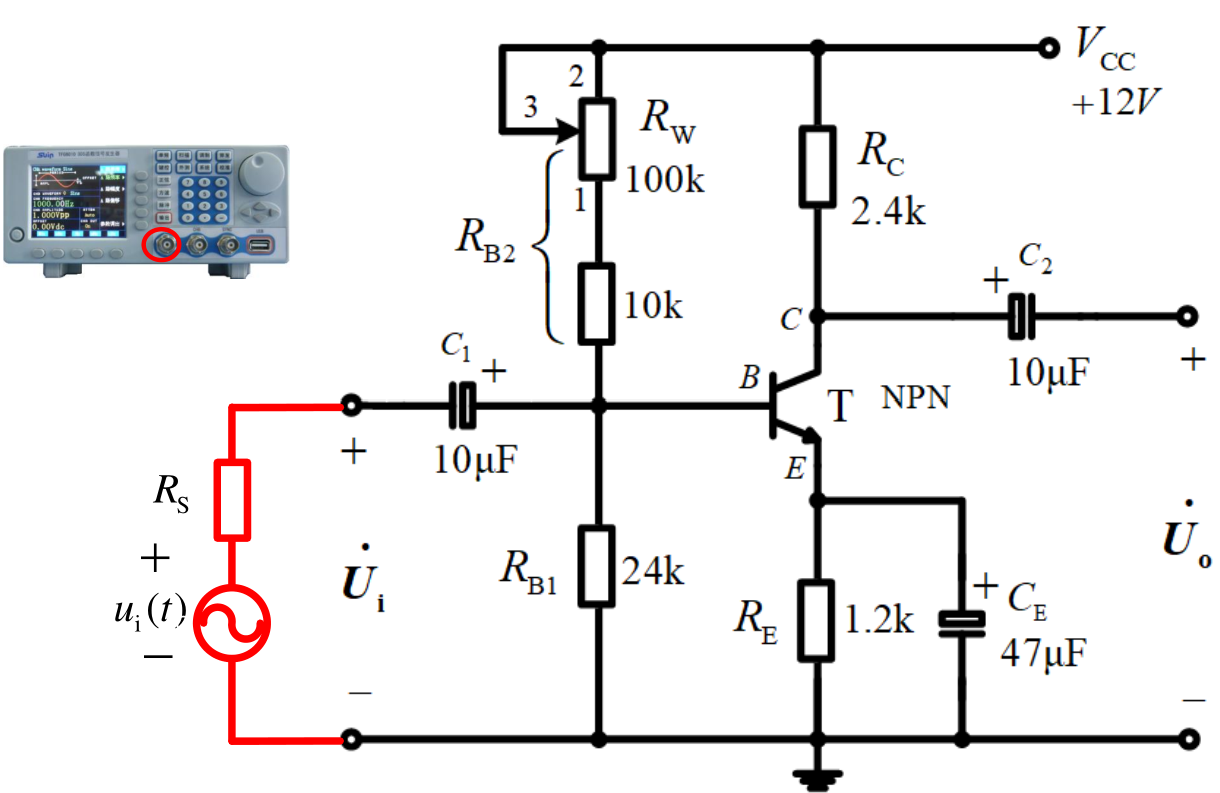
\includegraphics[height=150pt]{exp5}\\
        {\small 图八:实验电路}
    \end{center}

    \subsection{实验数据与误差分析}\label{subsec:19}
    \begin{figure*}[htb]
        \centering
        \subfloat[截止失真]{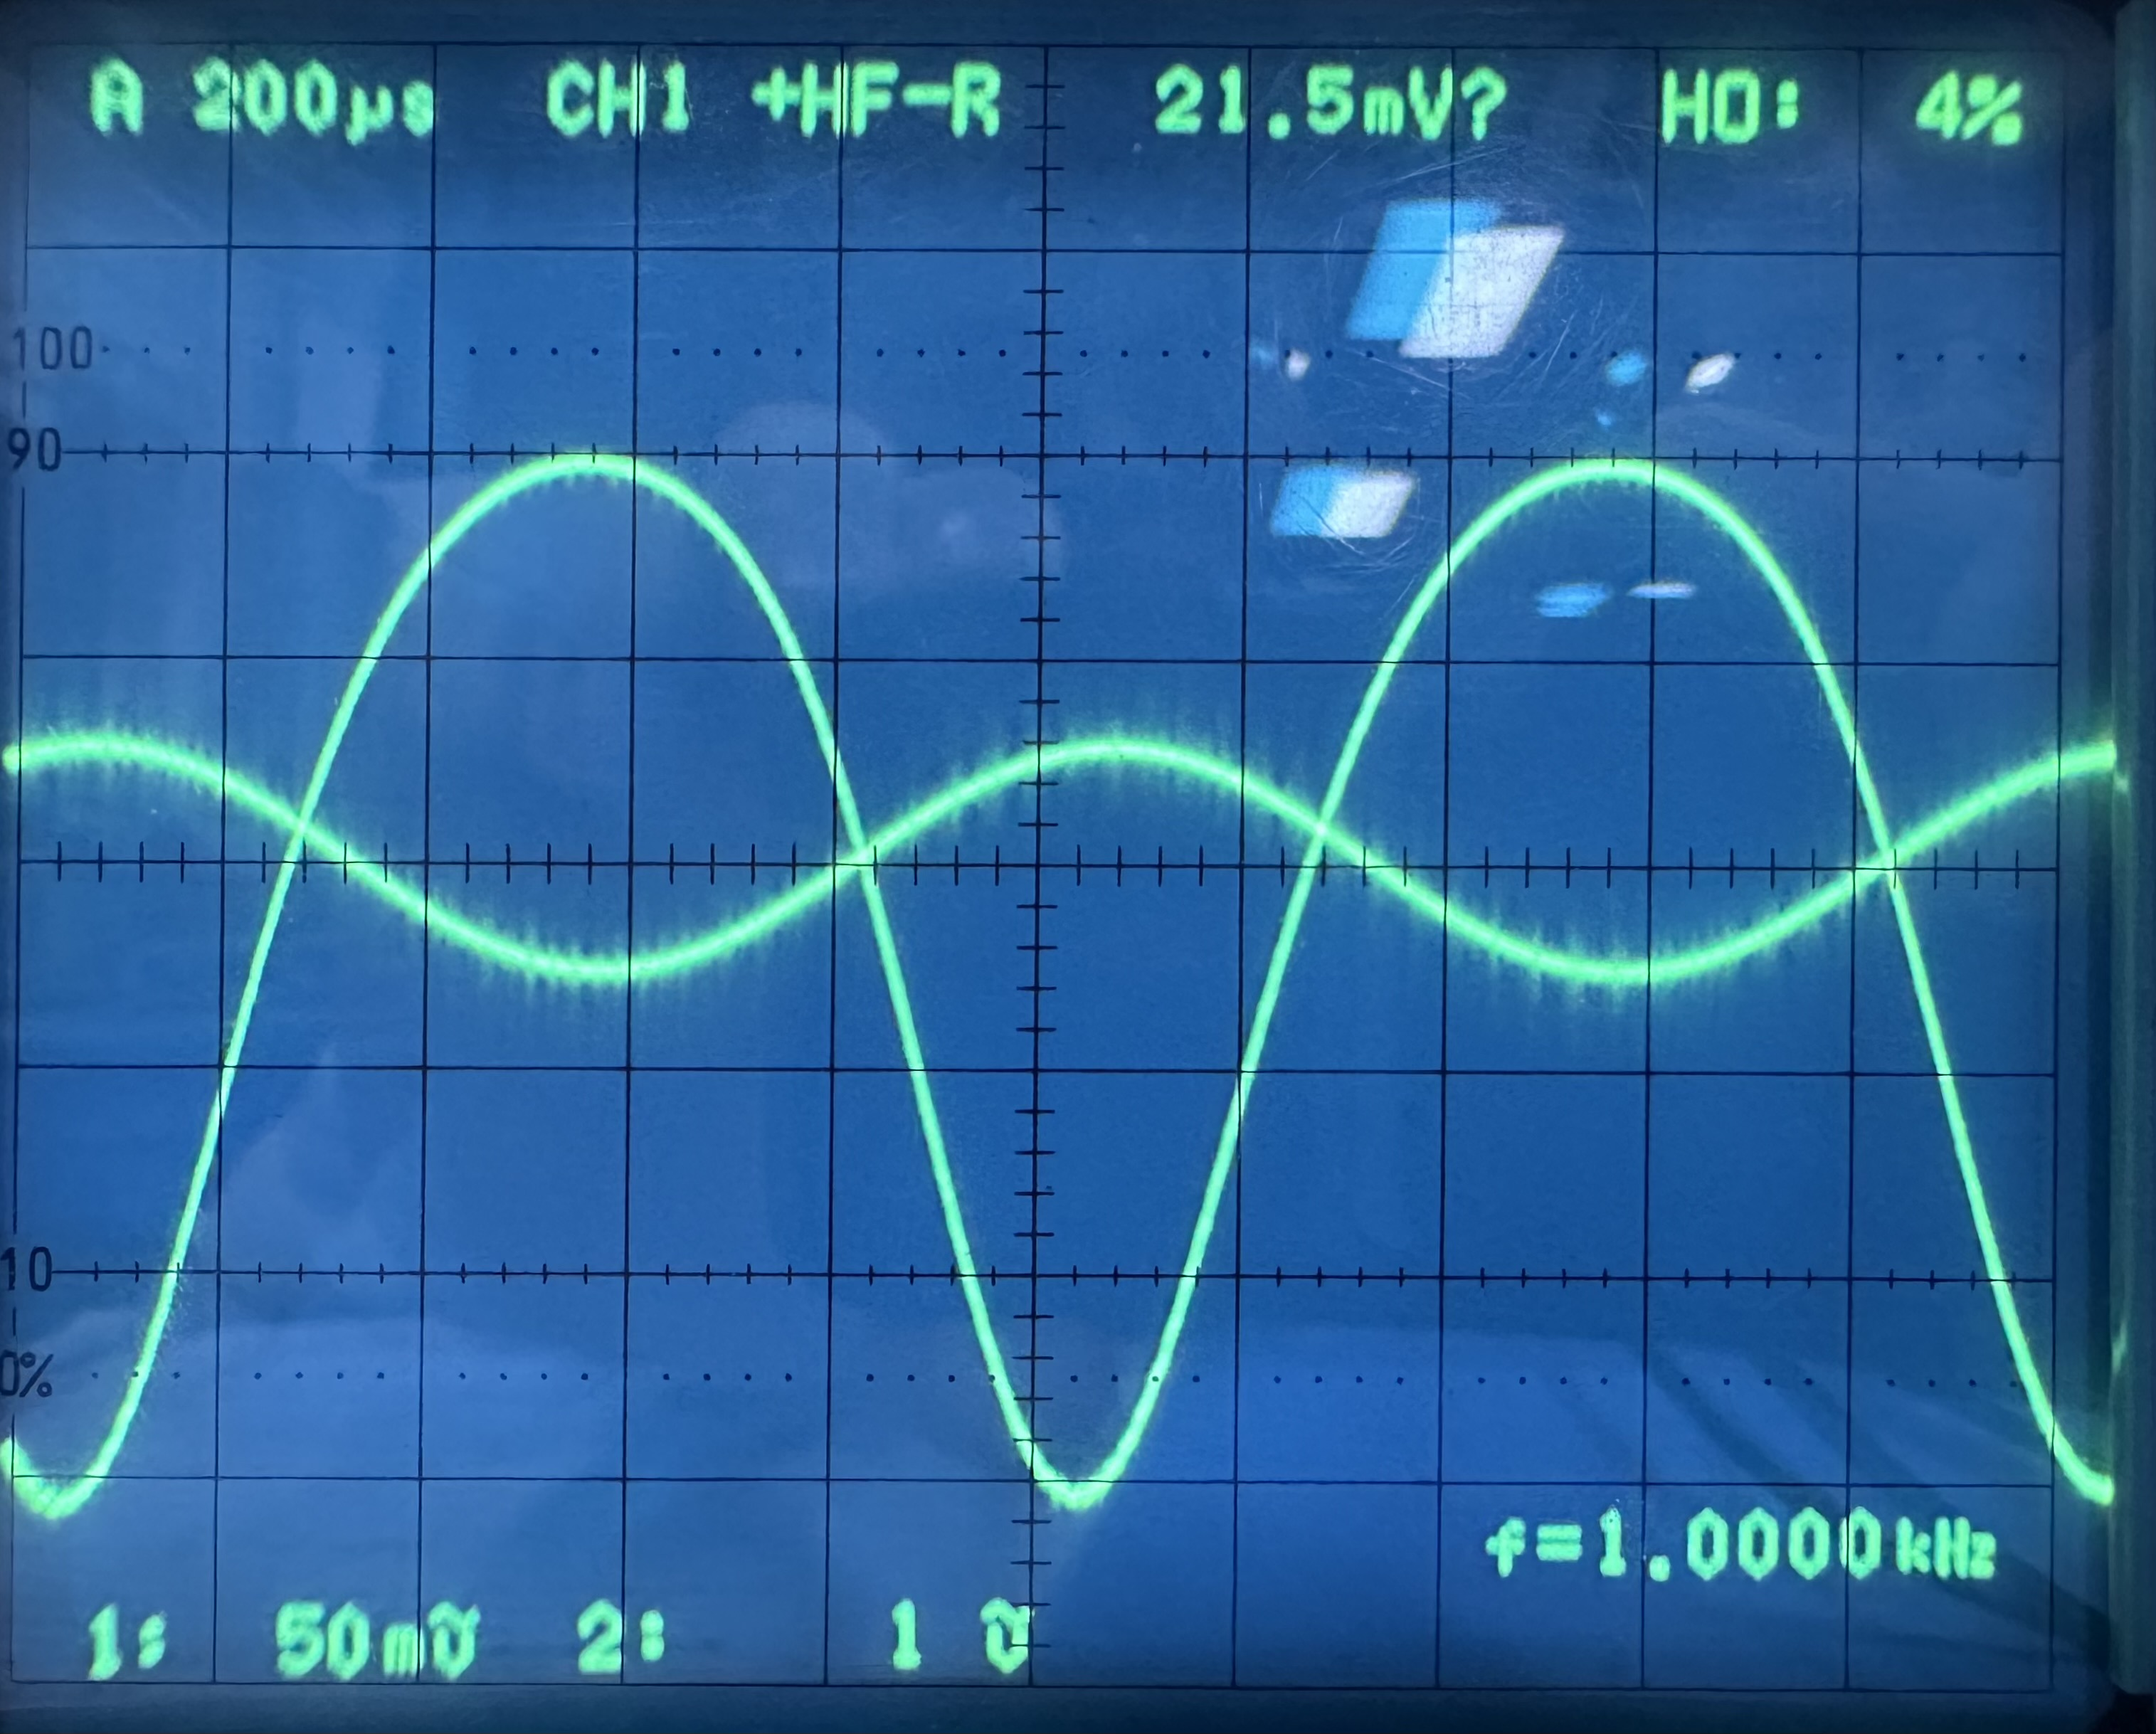
\includegraphics[height=120pt]{TD}}
        \subfloat[不失真]{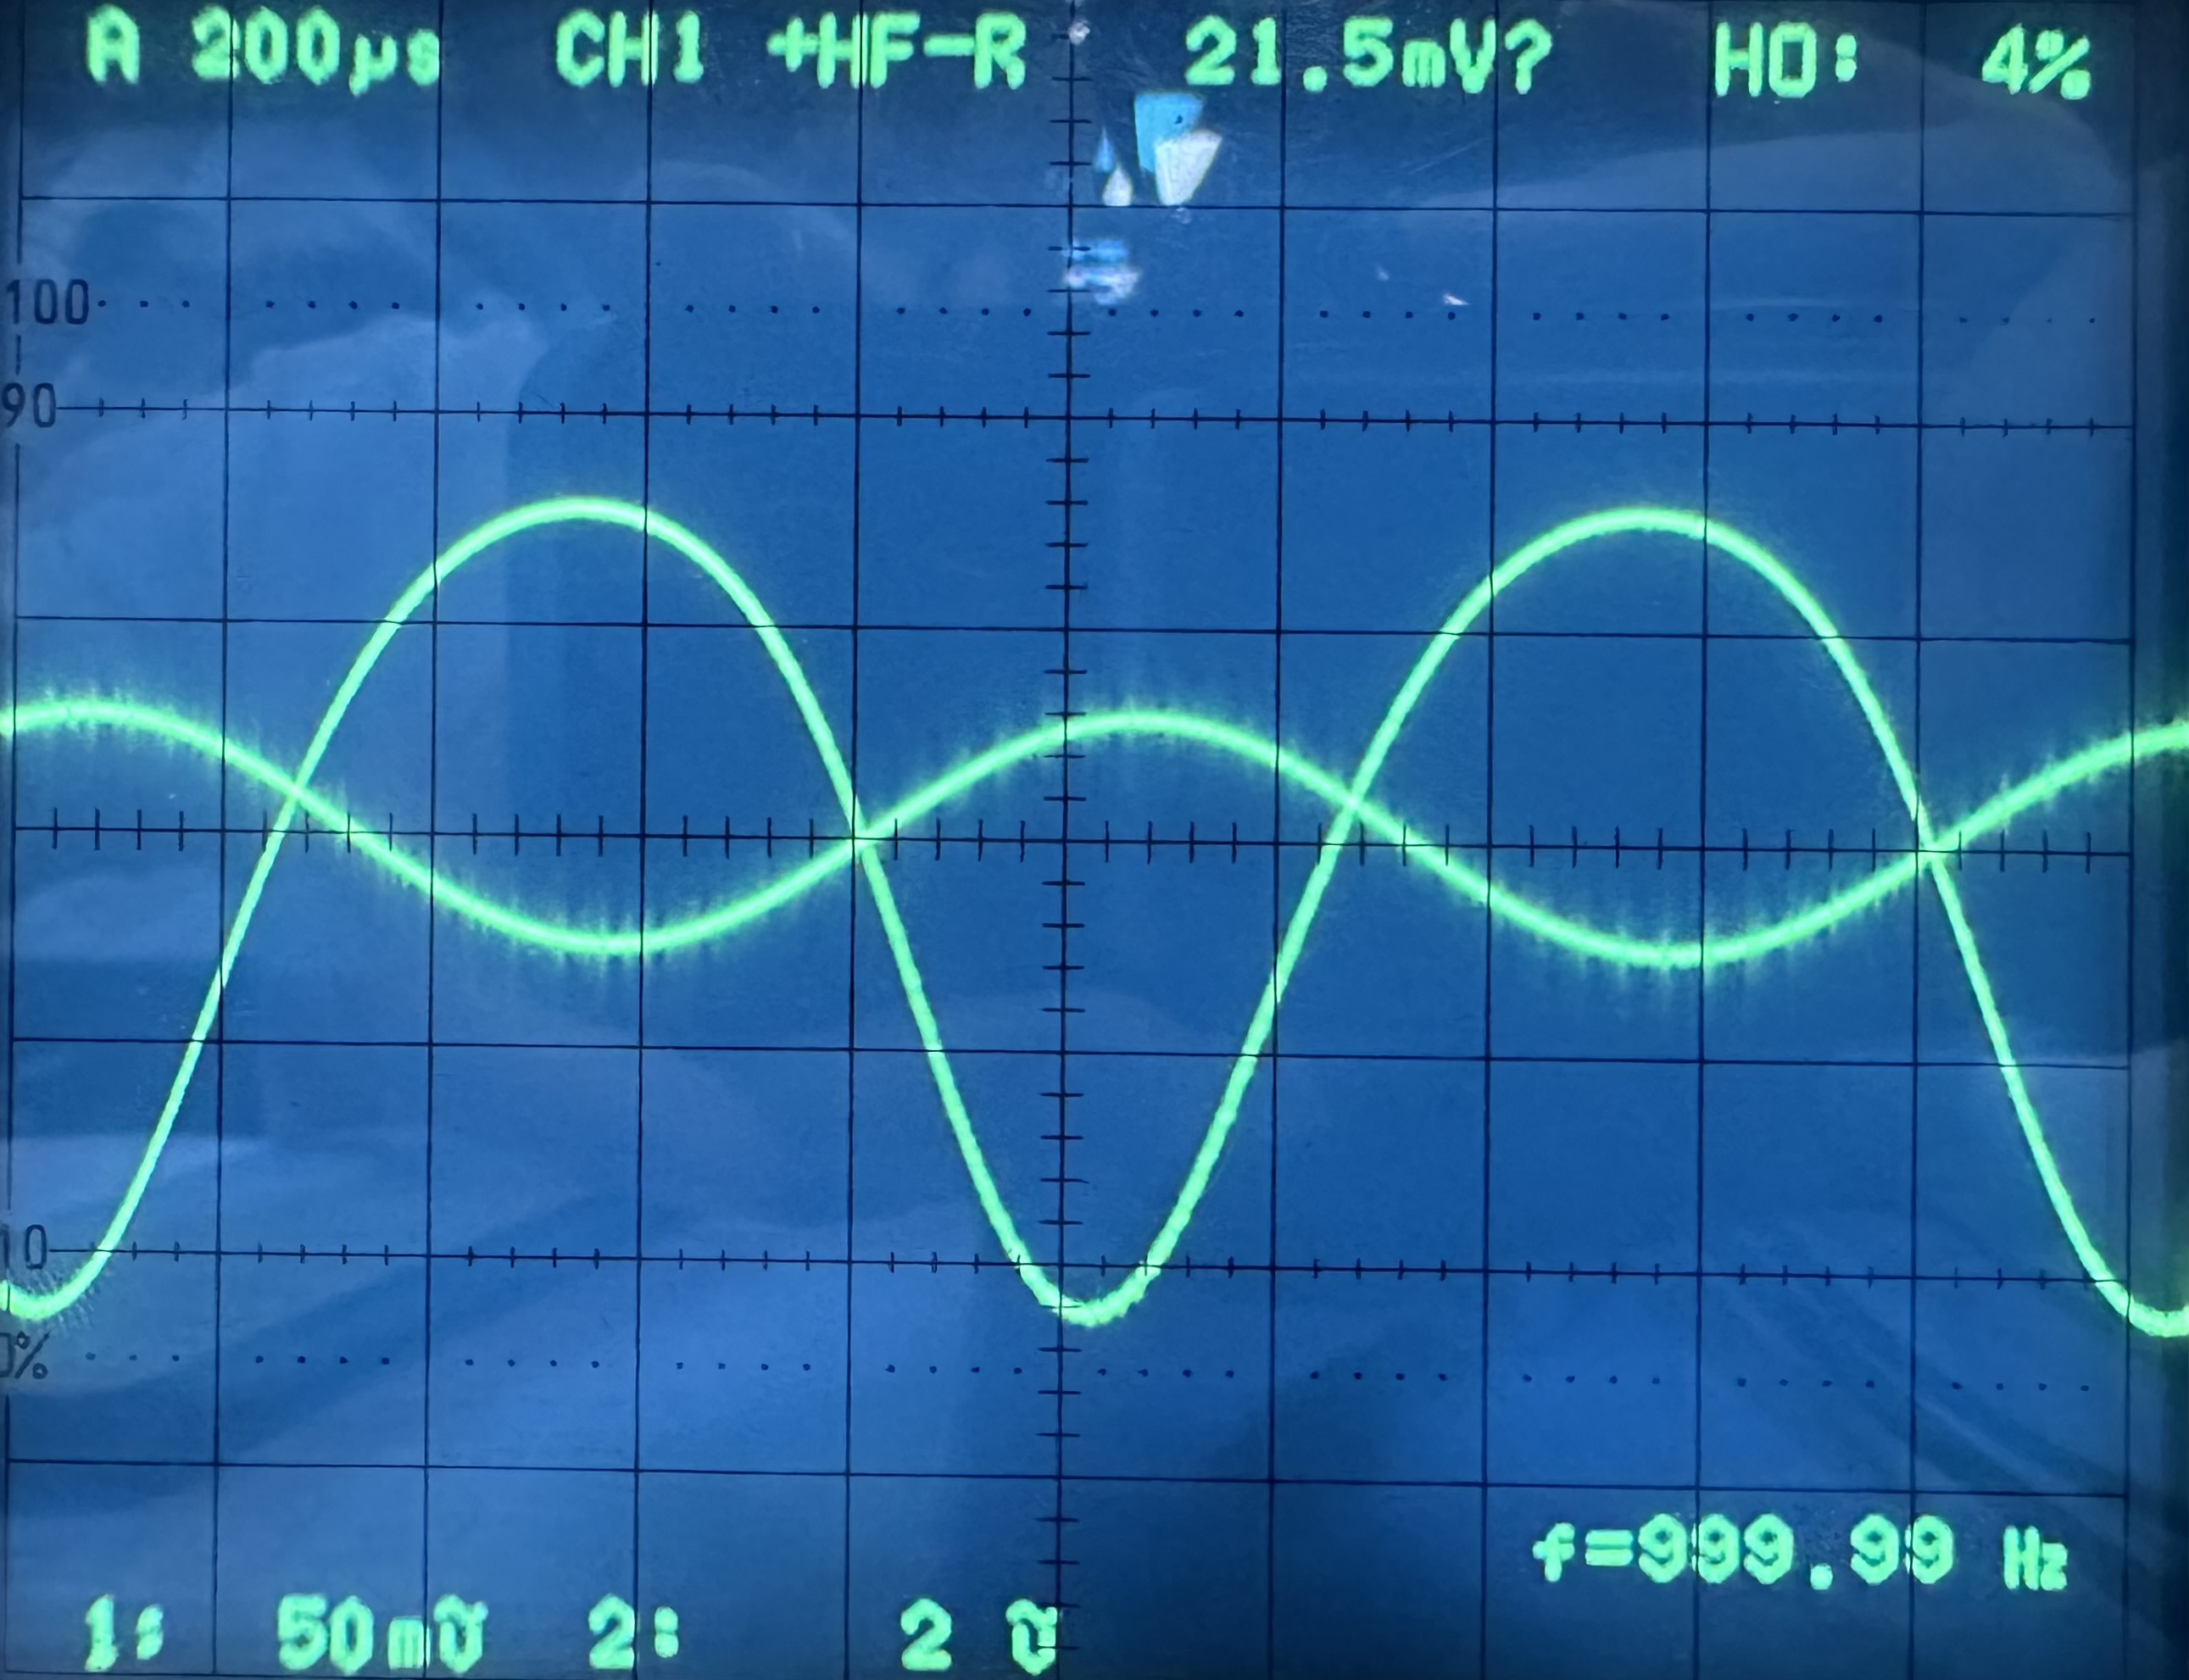
\includegraphics[height=120pt]{O}}
        \subfloat[饱和失真]{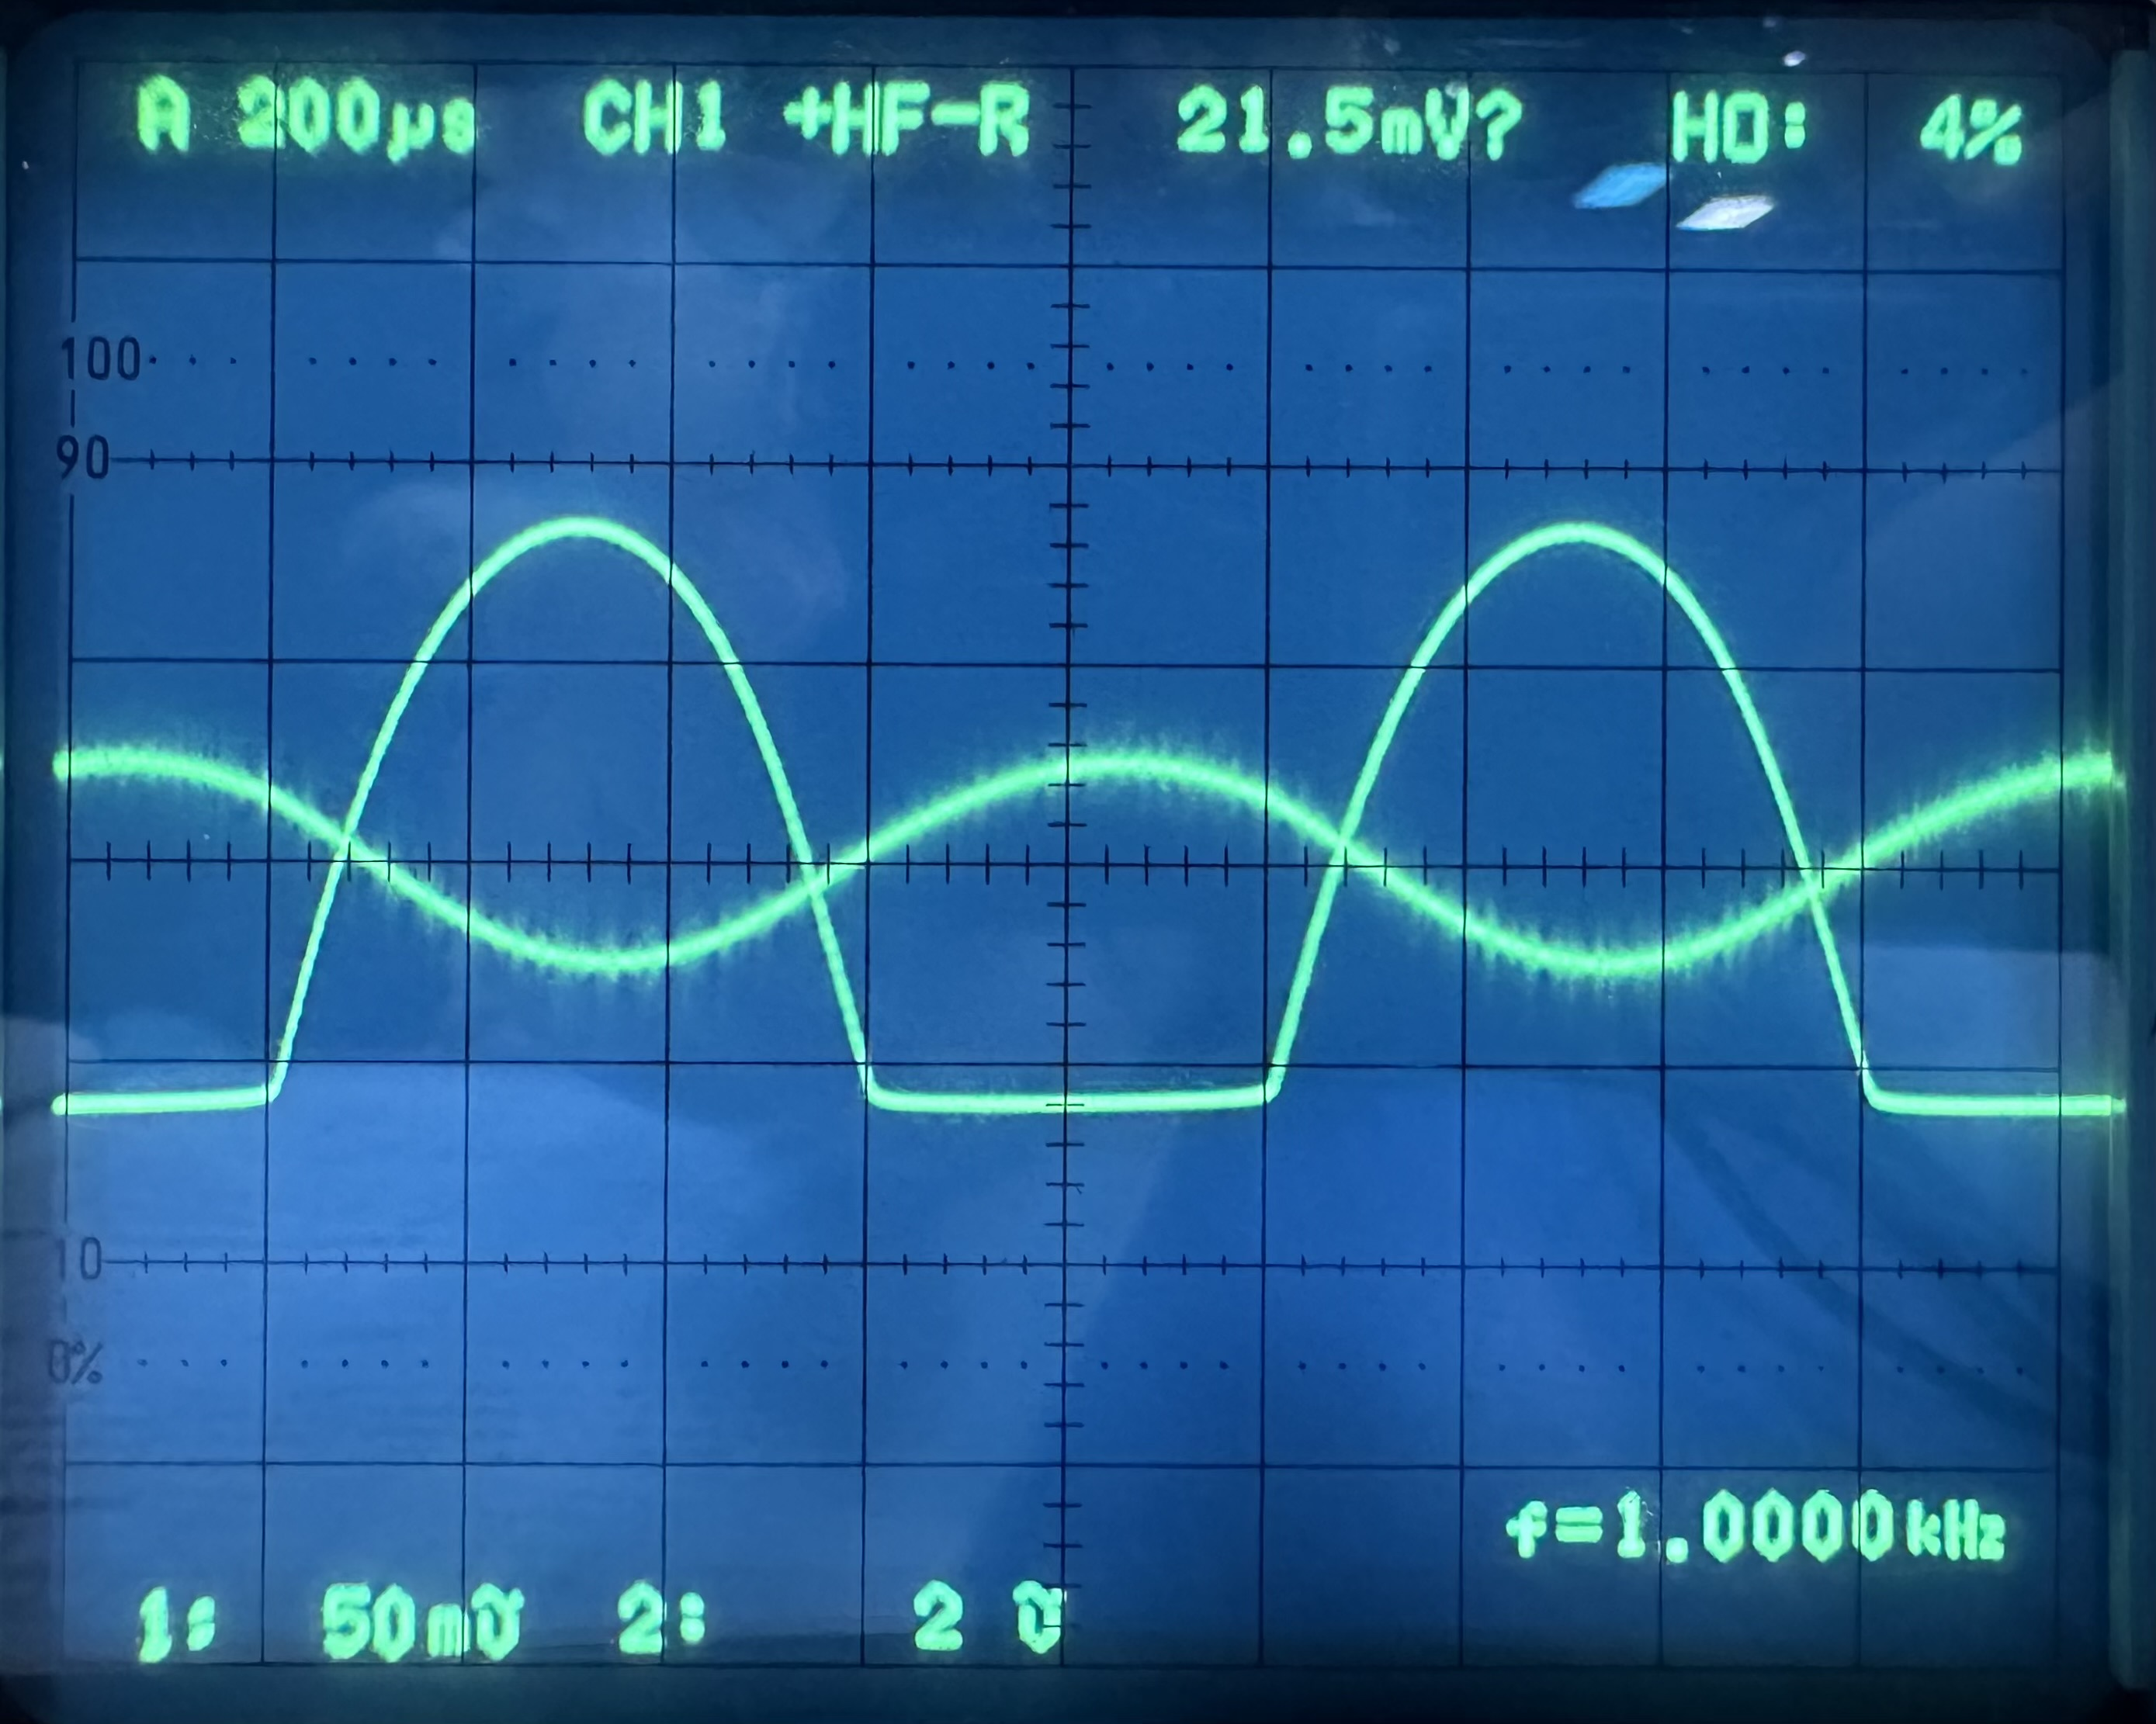
\includegraphics[height=120pt]{BD}}
        {\small 图九:输出波形失真图像}
    \end{figure*}

    \subsection{注意事项}\label{subsec:20}


    \section{思考题}\label{sec:8}


    \section{实验总结}\label{sec:9}

    \bibliography{main}
    \bibliographystyle{plain}

\end{document}
